\subsection{Questionnaire}
\subsubsection{System Usefulness}

A strong and significant main effect of the interaction device was found on the \textsc{system usefulness} $(Z(1) = -3.517, p = .000437, r = .622)$.. The medians for the keyboard and leap modes were 6.8125 and 1.8125 respectively. See figure~\ref{fig:system_usefulness}.

\begin{figure}[H]
\centering
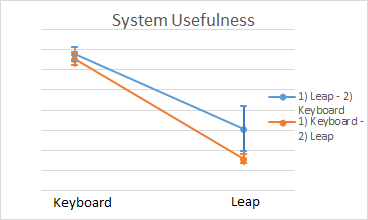
\includegraphics[width=0.5\textwidth]{imgs/results/system_usefulness}
\caption{System Usefulness - the mean and the 95\% intervals are plotted for both modes. The plots was split on the order of the interaction device. There is only a main effect of interaction device and no interaction device x order interaction effect.}
\label{fig:system_usefulness}
\end{figure}

\subsubsection{Interface Quality}

A strong and significant main effect of the interaction device was found on the \textsc{interface quality} $(Z(1) = -3.417, p = .000632, r = .604)$. The medians for the keyboard and leap modes were 6.167 and 3.833 respectively. See figure~\ref{fig:interface_quality}.

\begin{figure}[H]
\centering
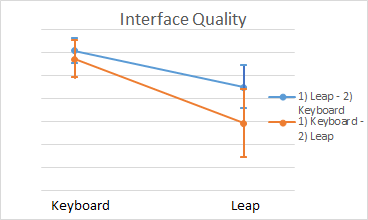
\includegraphics[width=0.5\textwidth]{imgs/results/interface_quality}
\caption{Interface Quality - the mean and the 95\% intervals are plotted for both modes. The plots was split on the order of the interaction device. There is only a main effect of interaction device and no interaction device x order interaction effect.}
\label{fig:interface_quality}
\end{figure}
